\centerline{\bf \huge 10 класс}
\centerline{\bf \huge Решения}

\problem{10.1}
Вася написал на доске несколько различных двузначных чисел. Оказалось, что сумма никаких двух из написанных на доске чисел не равна 90. Какое максимальное количество чисел мог написать Вася?

\textit{Ответ: 55.}

\textit{Решение.}
Заметим, что из каждой из 35 пар чисел $10-80,11-79,12-78, \ldots, 44-46$ на доске могло быть записано не более одного числа. Значит, по крайней мере 35 двузначных чисел из всех двузначных (от 10 до 99 ) не будут написаны. То есть на доске будет написано не более $90-35=55$ чисел.
Если на доске написать числа $45,46,47, \ldots, 99$, то сумма никаких двух из них не равна 90, а этих чисел 55.

\problem{10.2}
Дан квадратный трёхчлен $f(x)$. Известно, что существуют пары различных чисел $(m, k)$ таких, что $\frac{f(m)}{f(k)}=\frac{m}{k}$. Назовем такие пары хорошими. Докажите, что значение выражения $m \cdot k$ во всех хороших парах одинаково.

\textit{Решение.}
Пусть $f(x)=a x^2+b x+c(a \neq 0)$. Тогда $\frac{f(m)}{f(k)}=\frac{a m^2+b m+c}{a k^2+b k+c}=\frac{m}{k}$. Домножив на знаменатели, получим $a m^2 k+b m k+c k=a k^2 m+b k m+c m$. Это равенство можно преобразовать к виду $(a m k-c)(m-k)=0$. Так как $m \neq k$, то $a m k=c$, откуда произведение $m k=\frac{c}{a}-$ одинаковое для любой пары.

\problem{10.3}
На доске были написаны не обязательно разные неотрицательные целые числа. Коля вычел из каждого исходного числа 1 , затем сложил модули всех получившихся чисел, и получил сумму $S_1$. Вася вычел из каждого исходного числа на доске 2 , затем сложил модули всех получившихся чисел, и получил сумму $S_2$ Наконец Андрей вычел из каждого исходного числа на доске 3 , затем сложил модули всех получившихся чисел, и получил сумму $S_3$. Сколько двоек было написано на доске?

\textit{Ответ: $\frac{S_3-2 S_2+S_1}{2}$.}

\textit{Решение.} 
Пусть сумма всех чисел на доске равна $S$, их количество равно $n$, а количества нулей, единиц, двоек на доске равны соответственно $a, b, c$. Тогда $S_1=S-n+2 a$, так как каждое число, отличное от нуля, уменьшилось на 1 , а ноль, напротив, превратился в единицу, то есть оказался на 2 больше, чем $0-1$. Так же $S_2=S-2 n+4 a+2 b$, так как каждое число, отличное от нуля и единицы, уменьшилось на 2 , а ноль, напротив, превратился в двойку, а единица превратилась в единицу. Наконец, аналогично, $S_3=S-3 n+6 a+4 b+2 c$. Отсюда можно получить, что $c=\frac{S_3-2 S_2+S_1}{2}$.


\problem{10.4}
Есть 30 нечётных натуральных чисел. Оказалось, что их можно разбить на 10 троек так, что в каждой тройке одно из чисел равно произведению двух других. Может ли сумма этих 30 чисел равняться 2024?

\textit{Ответ: Не может.}

\textit{Решение.}
Предположим, что описанная ситуация возможна. Пусть в одной из троек будут числа $a, b, a b$. Тогда их сумма есть $a+b+a b=(a+1)(b+1)-1$. Так как числа $a, b-$ нечётные, то произведение $(a+1)(b+1)$ делится на 4 , как произведение двух чётных чисел. Тогда $a+b+a b=4 k-1$. Пусть в $i$-й тройке ( $i=1,2, \ldots, 10$ ) сумма равна $4 k_i-1$. Тогда сумма всех 30 чисел равна $\left(4 k_1-1\right)+\left(4 k_2-1\right)+\ldots+\left(4 k_{10}-1\right)=4 M-10$. Но $4 M-10 \neq 2024$, так как число 2034 не делится на 4. Противоречие.

\problem{10.5}
В трапеции $A B C D$ длина боковой стороны $A B$ равна сумме длин оснований. Окружность $\Omega$ с центром в точке $A$, проходящая через $D$, пересекает отрезки $B D$ и $B A$ в точках $E$ и $F$ соответственно. Докажите, что точки $B, C, E, F$ лежат на одной окружности.


\begin{wrapfigure}{r}{0.5\linewidth}     
    \vspace{-7mm}
    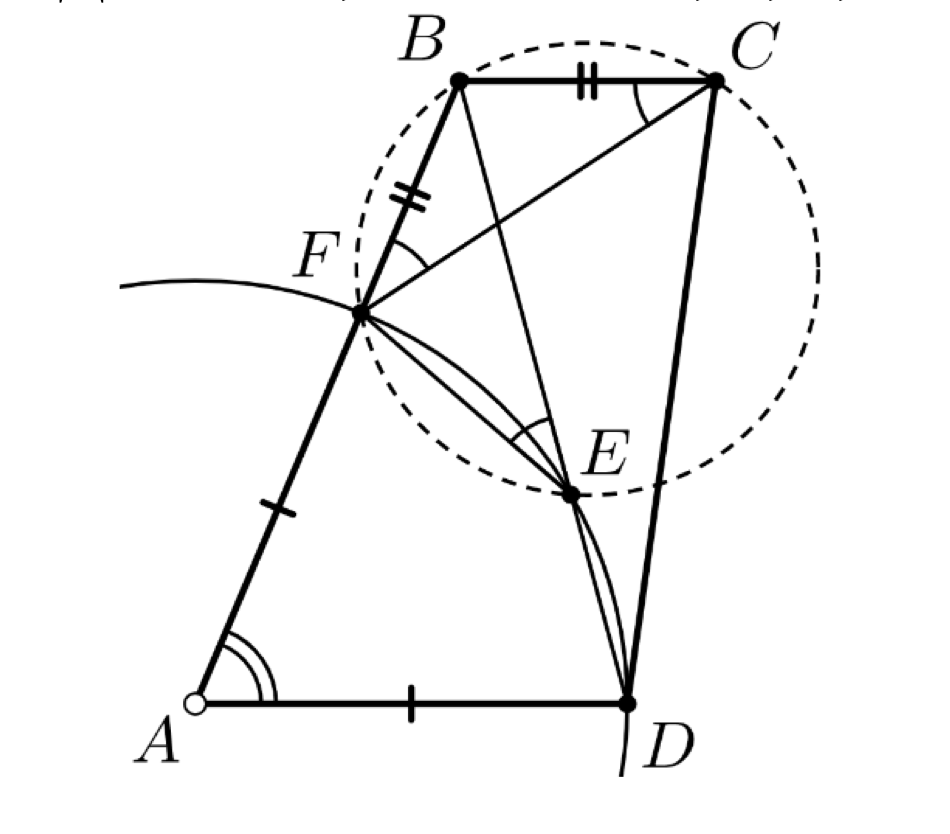
\includegraphics[width=\linewidth]{ЭлМШ 2025-2026/III блок/10/Тренировки/III/Решения/10.3.5.png}
\end{wrapfigure}

\textit{Решение.}
Так как $A B=A D+B C$ и $A F=A D$, то $B F=B C$ и треугольник $B F C$ равнобедренный. Обозначим $\angle B A D=2 \alpha$. В окружности $\Omega$ угол $F E D$ вписанный, а соответствующий ему центральный угол равен $360^{\circ}-2 \alpha$, поэтому $\angle F E D=180^{\circ}-\alpha$ и смежный с ним $\angle F E B=\alpha$. Основания $B C$ и $A D$ трапеции параллельны, значит, $\angle A B C= 180^{\circ}-2 \alpha$, а раз треугольник $B F C$ равнобедренный, то $\angle B C F=\angle B F C=\alpha$. Таким образом, $\angle B C F=\angle B E F$, а значит, точки $B, C, E, F$ лежат на одной окружности.